
%%%%%%%%%%%%%%%%%%%%%%%%%%%%%%%% FUNCTIONAL SUMMARIES


\frame{
\frametitle{}
\begin{block}{}
\centering
Functional Summaries and Their Confidence Sets
\end{block}
}

\frame{
    \frametitle{Applications (of Functional Summaries)}

\begin{columns}
    \column{.45\textwidth}
    \begin{block}{One Sample of Summaries}
        \begin{itemize}
            \item Variance
            \item Mean Computation
            \item Confidence Bands
            \item Functional Boxplots
        \end{itemize}
    \end{block}
    \column{.45\textwidth}
    \begin{block}{Two Samples of Summaries}
        \begin{itemize}
            \item Two-sample Hypothesis Test
            \item Paired Hypothesis Test
            \item Clustering
            \item Classification
        \end{itemize}
    \end{block}
\end{columns}
}

\frame{
\frametitle{Eyeballing the Distribution}

\begin{block}{}
  \centering
  \only<1>{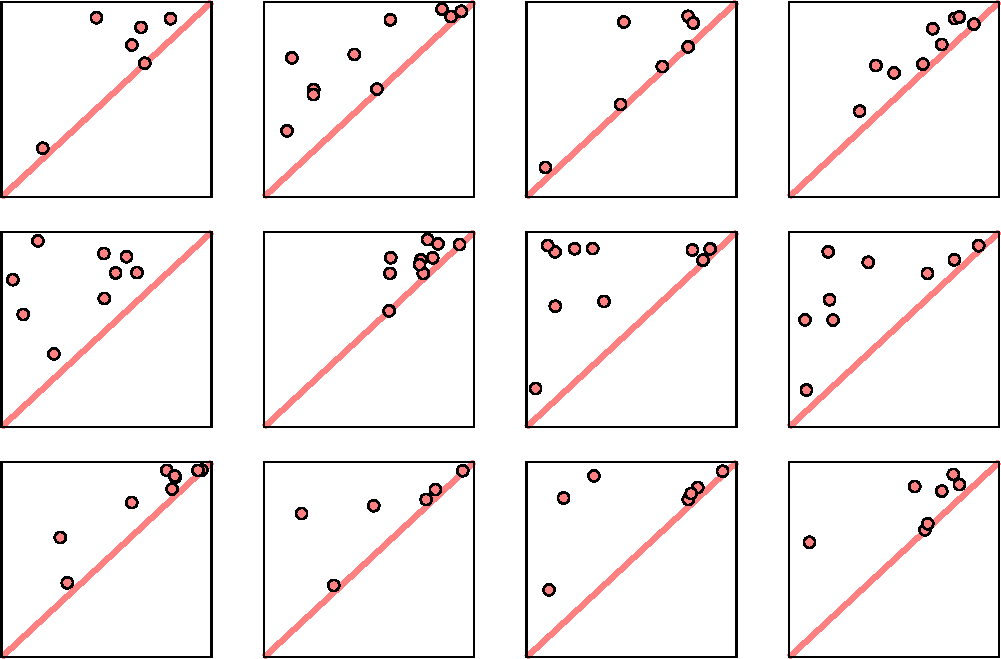
\includegraphics[height=2in]{stat/sampling-dgms}}%
  \only<2>{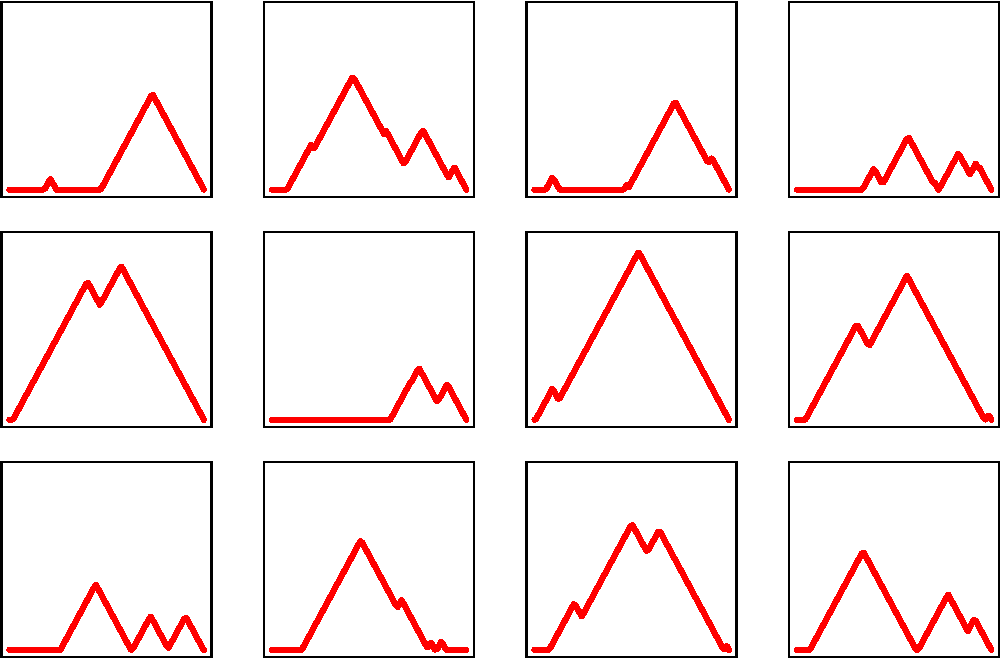
\includegraphics[height=2in]{stat/sampling-lscapes}}%
\end{block}

}

\frame{
\frametitle{Persistence Landscapes}
\framesubtitle{
    \onslide<3->{    Bubenik. Statistical Topological Data Analysis using
    Persistence Landscapes.
JMLR, 2015.}}

\begin{center}
\only<1>{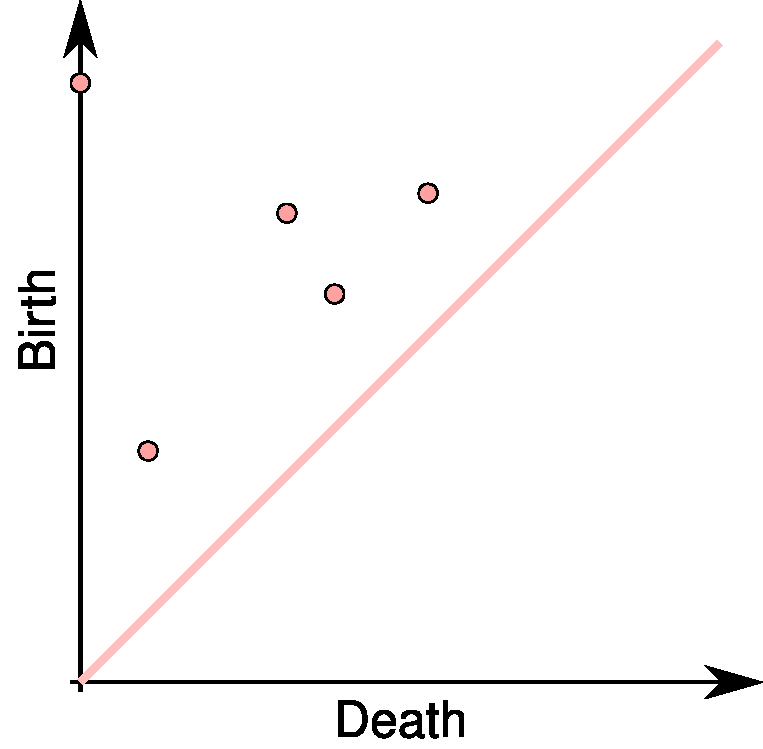
\includegraphics[height=2in]{stat/persistence-dgm}}%
\only<2>{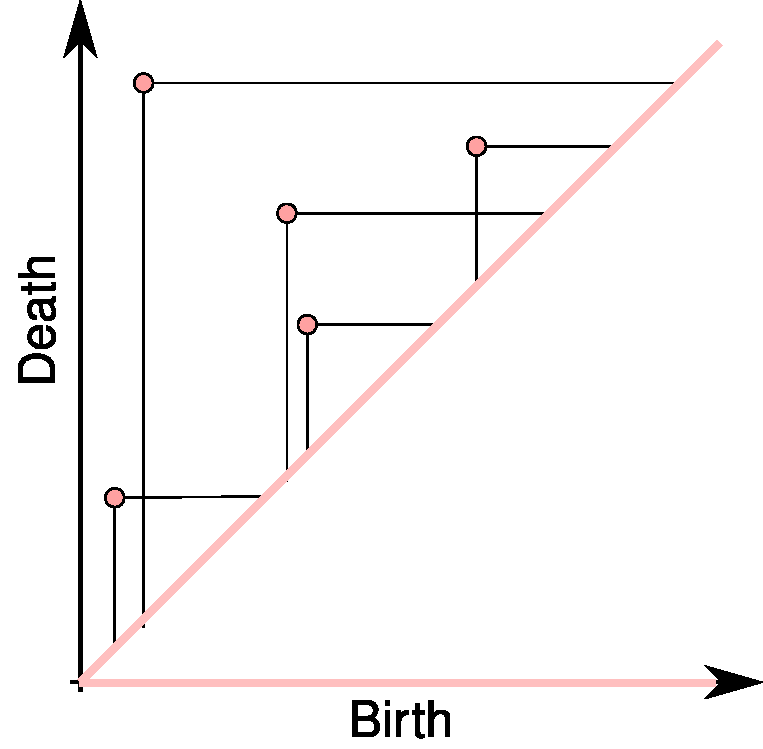
\includegraphics[height=2in]{stat/persistence-dgm-dropped}}%
\only<3>{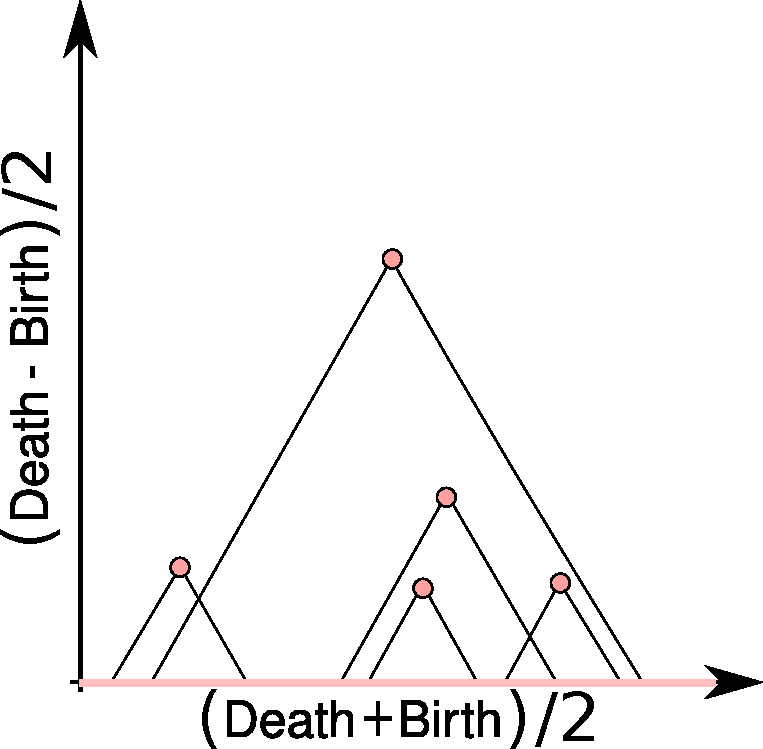
\includegraphics[height=2in]{stat/persistence-landscape}}%
\only<4>{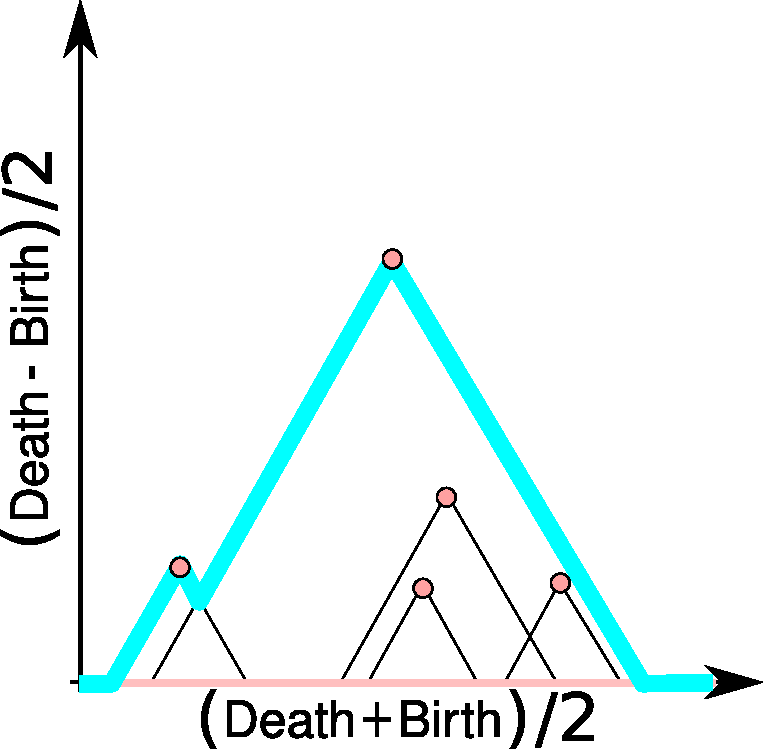
\includegraphics[height=2in]{stat/persistence-one-landscape}}%
\only<5->{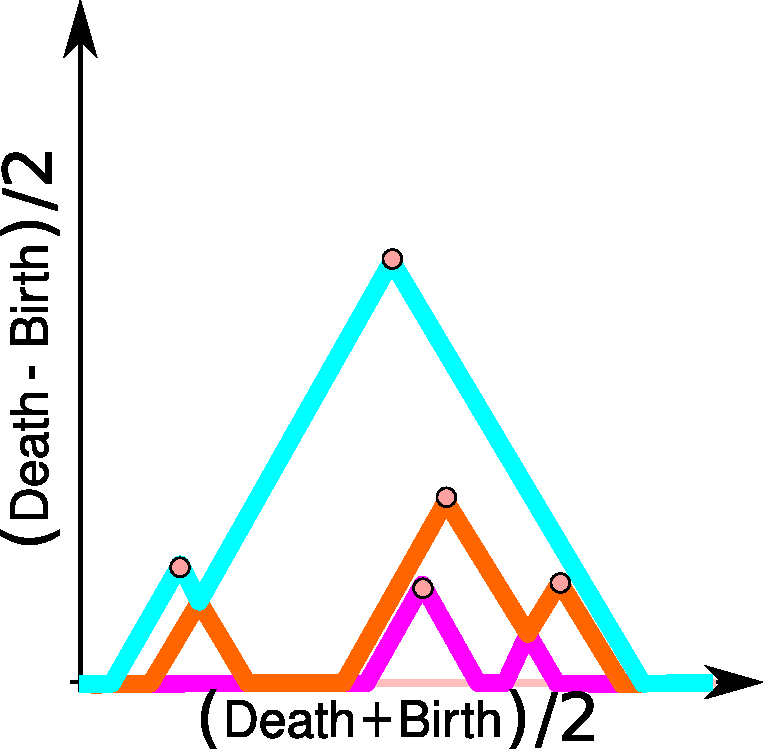
\includegraphics[height=2in]{stat/persistence-all-landscapes}}%
\end{center}
}

\frame{
    \frametitle{Persistence Landscapes and Silhouettes}
\begin{columns}
    \column{.45\textwidth}
    \begin{center}

        \only<1>{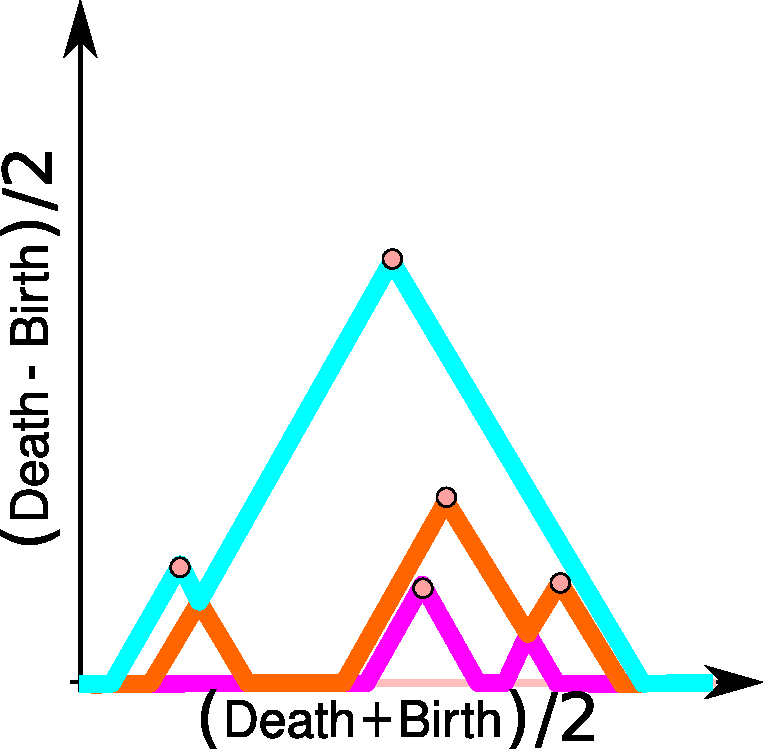
\includegraphics[height=2.5in]{stat/persistence-all-landscapes}}%
        \only<2->{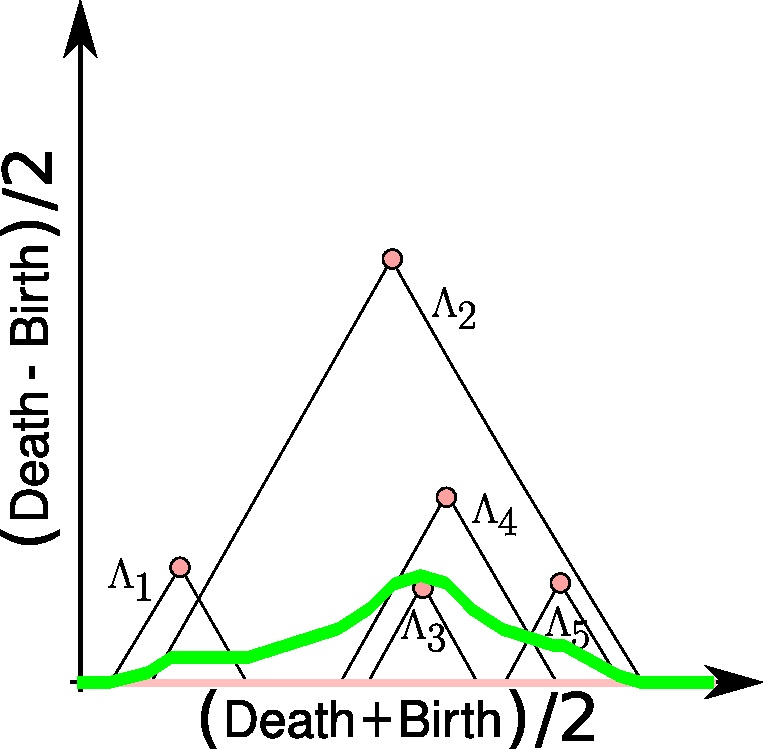
\includegraphics[height=2.5in]{stat/persistence-silhouette}}%
    \end{center}
    \column{.45\textwidth}

    \only<1>{
        \begin{block}{}
            $$\Lambda \colon \R \times \Z_{+} \to \R$$
            $$\Lambda_i(\cdot) := \Lambda(\cdot,i)$$
        \end{block}
    }

    \only<2->{
        \begin{block}{Weighted Silhouette}
            $$ \phi(t) = \frac{\sum_{i=1}^n w_i \Lambda_i(t) }{ \sum_{j=1}^n w_j} $$
        \end{block}
        \onslide<3>{
            \begin{block}{Power-Weighted Silhouette}
            $$w_i = |d_i - b_i|^p$$
            \end{block}
        }
    }%end only<4->

\end{columns}


}

\frame{
    \frametitle{Weak Convergence of Landscapes}

\begin{columns}
    \column{.45\textwidth}
    \begin{center}
        \only<1>{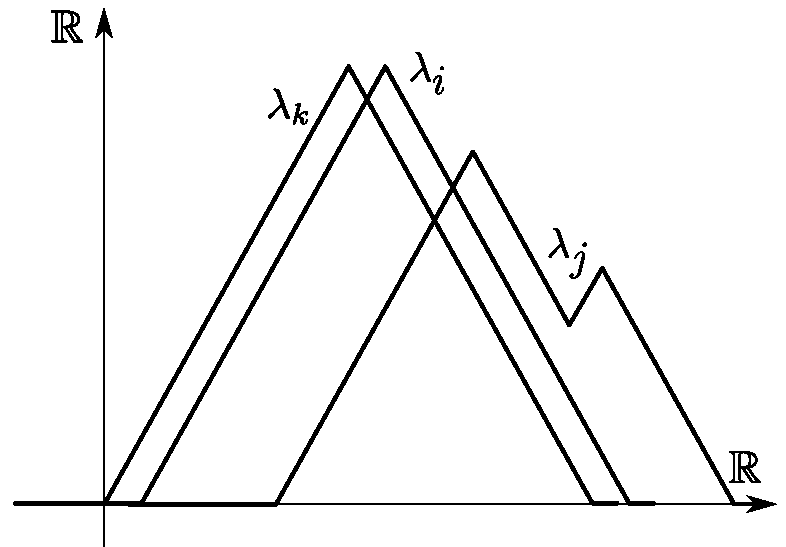
\includegraphics[width=\textwidth]{stat/gaussianprocess-lscapes}}%
        \only<2>{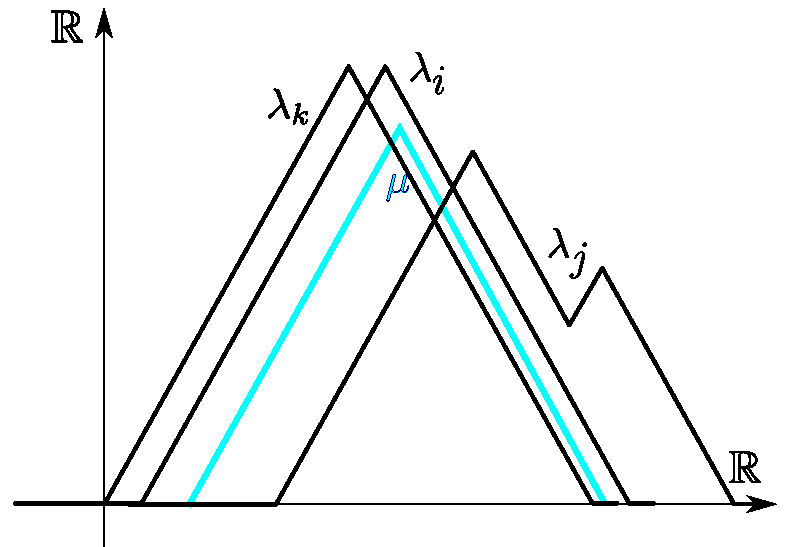
\includegraphics[width=\textwidth]{stat/gaussianprocess-mean}}%
        \only<3>{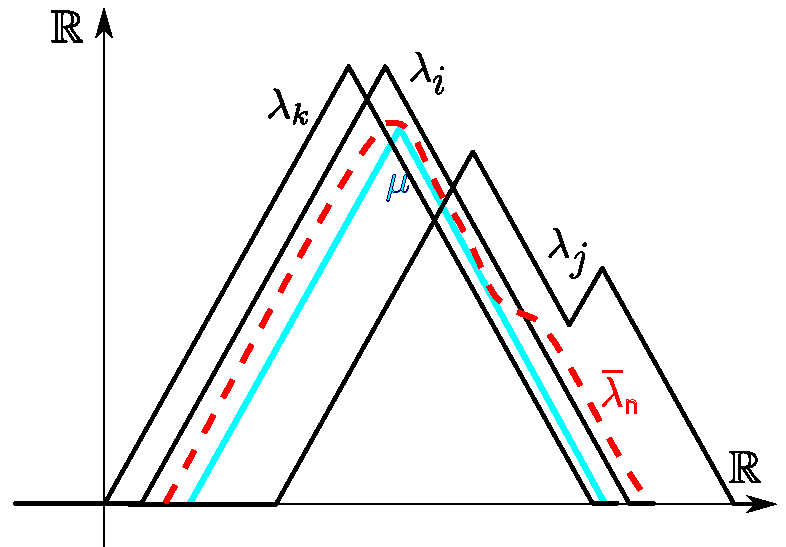
\includegraphics[width=\textwidth]{stat/gaussianprocess-empirical}}%
        \only<4->{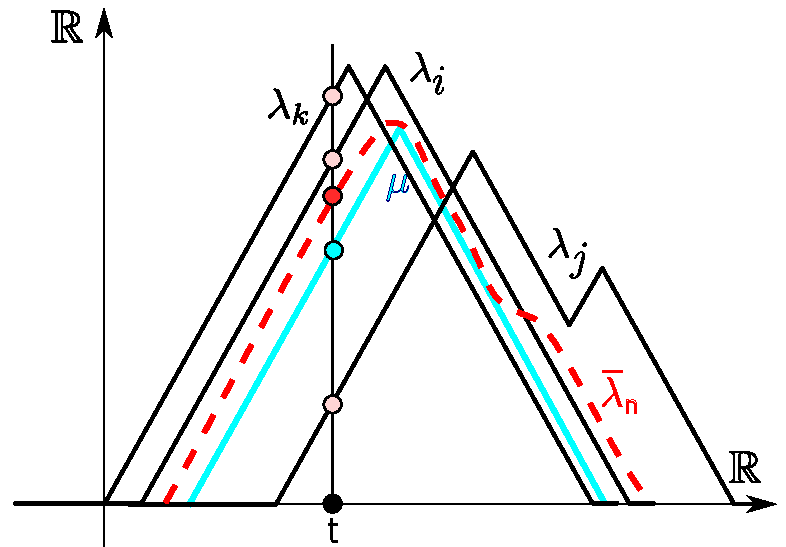
\includegraphics[width=\textwidth]{stat/gaussianprocess}}%
    \end{center}
    \column{.45\textwidth}
    \begin{block}{}
        Let $\lambda_1, \ldots, \lambda_n \sim \mathcal{L}_T$.\\ \pause
        $\lambda$ : true (unknown) landscape\\
        $\mu = \mathbb{E}(\lambda_i)  $\\ \pause
        $\bar{\lambda}_n$ : average landscape \pause
    \end{block}
\end{columns}

\begin{block}{Pointwise Convergence  [Bubenik-2015 (JMLR), also arXiv:1207.6437].}
    {\color{red} $\bar{\lambda}_n$} converges pointwise to {\color{cyan} $\mu$}.
\end{block} \pause

\begin{block}{Uniform CLT}
    We proved this in [CFLRW (SoCG 2014, JCG 2015), also arXiv:1312.0308].
\end{block}

} % end frame



\frame{
\frametitle{{Asymptotic} Confidence Bands}
 \begin{columns}
 \column{.45\textwidth}
    \begin{center}
    \only<0>{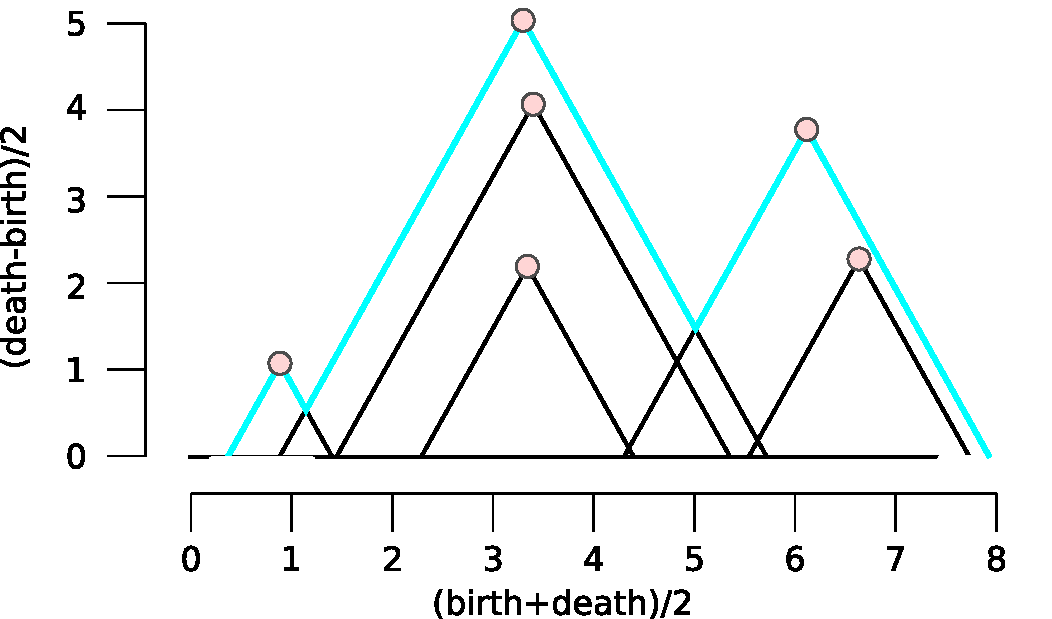
\includegraphics[width=\textwidth]{stat/triangles3b}}%
    \only<1-2>{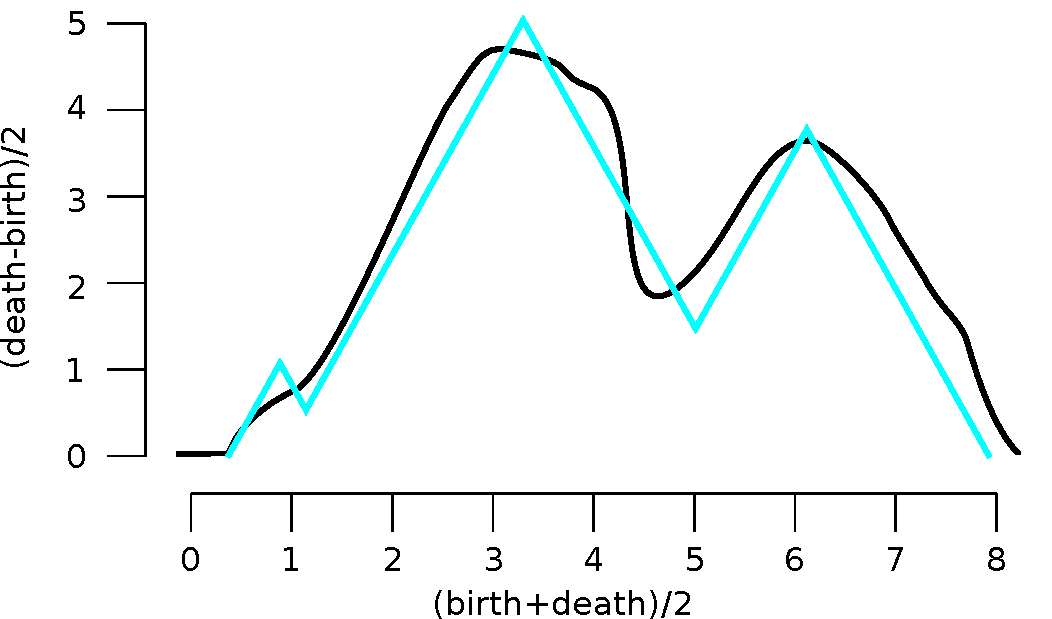
\includegraphics[width=\textwidth]{stat/triangles-avg}}%
    \only<3->{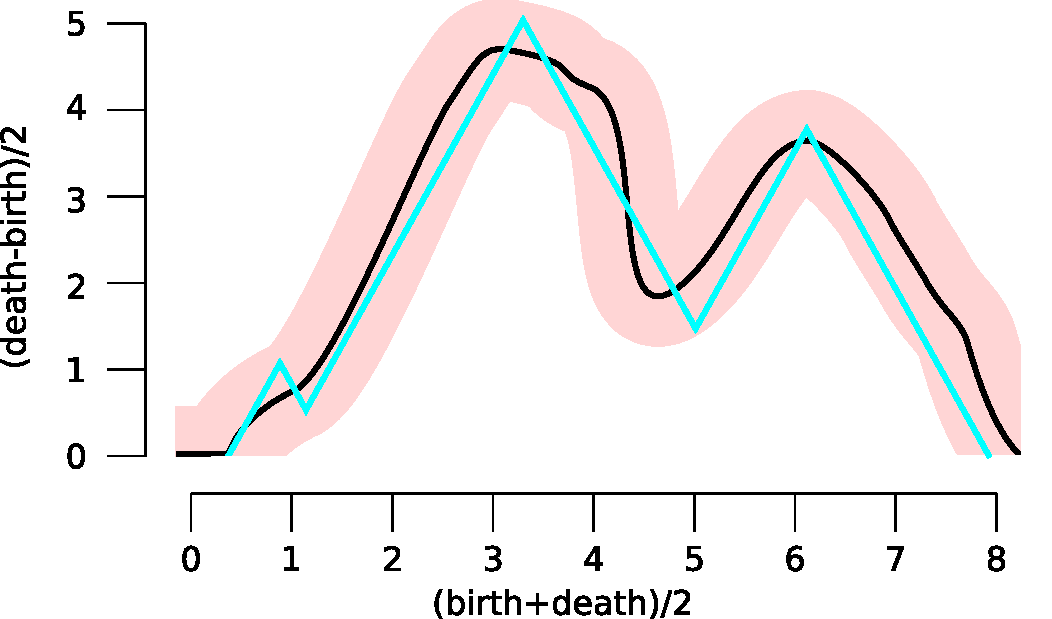
\includegraphics[width=\textwidth]{stat/triangles-CI}}%
    \end{center}
 \column{.45\textwidth}
    \begin{block}{}
    \begin{eqnarray*}
    \mathbb{E}||\lambda -\bar{\lambda}_n||_{\infty}
    &\leq&
    \overbrace{\mathbb{E}||\mu
    -\bar{\lambda}_n||_{\infty}}^{\text{variance}}\\
    \onslide<1>{&& + \underbrace{\mathbb{E}||\lambda - \mu
    ||_{\infty}}_{\text{bias}} \\ }
    \end{eqnarray*}
    \end{block}
 \end{columns}


\onslide<3->{
\begin{block}{\onslide<3->{Asymptotic} Confidence Band}
Find $c$ such that $\ell_n = \bar{\lambda}_n - c$ and
$u_n = \bar{\lambda}_n + c$ such that
$$
\only<3->{\lim_{n\to \infty}}
\mathbb{P}(\ell_n(t) \leq \mu(t) \leq u_n(t) \text{ for all } t)
\geq 1 - \alpha.
$$
\end{block}
}% end onslide
}% end frame


\frame<2>{
\frametitle{Confidence Bands for Landscapes}
\framesubtitle{Via the Multiplier Bootstrap}
\begin{block}{}
 $\xi_1, \ldots, \xi_n \sim N(0,1)$\\
 $$\widetilde{\mathbb{G}}_n(f_t) := \frac{1}{\sqrt{n}}
 \sum_{i=1}^n \xi_i (\lambda_i(t) - \bar{\lambda}_n (t))$$
\end{block}

\begin{columns}
\column{.45\textwidth}
  \begin{block}{$\alpha$-Quantile}
  $q^{\alpha}$ is the unique value such that
  $$
  \mathbb{P} \left( \sup_{t} | \widetilde{\mathbb{G}}_n(f_t) | >
q^{\alpha}  \Biggm| \{ \lambda_i \} \right) = \alpha
  $$
  \onslide<2->{*Approx. $\widetilde{Z}_{\alpha}$ by MC
simulation}
  \end{block}
\column{.45\textwidth}
  \only<1>{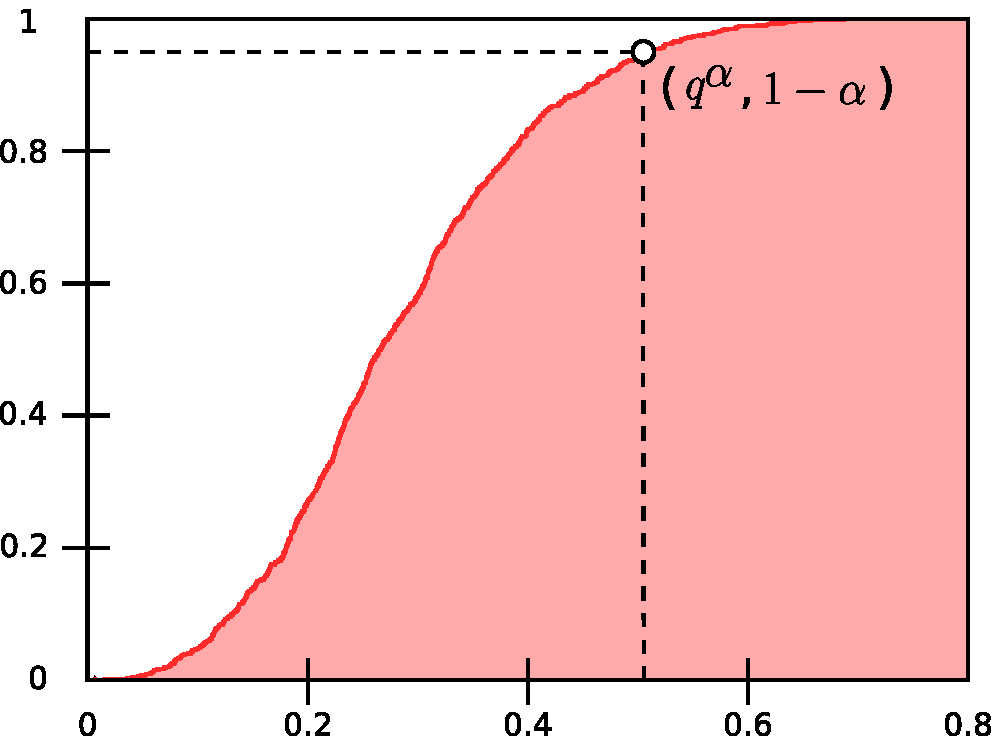
\includegraphics[width=0.75\textwidth]{stat/cdf-full}}%
  \only<2->{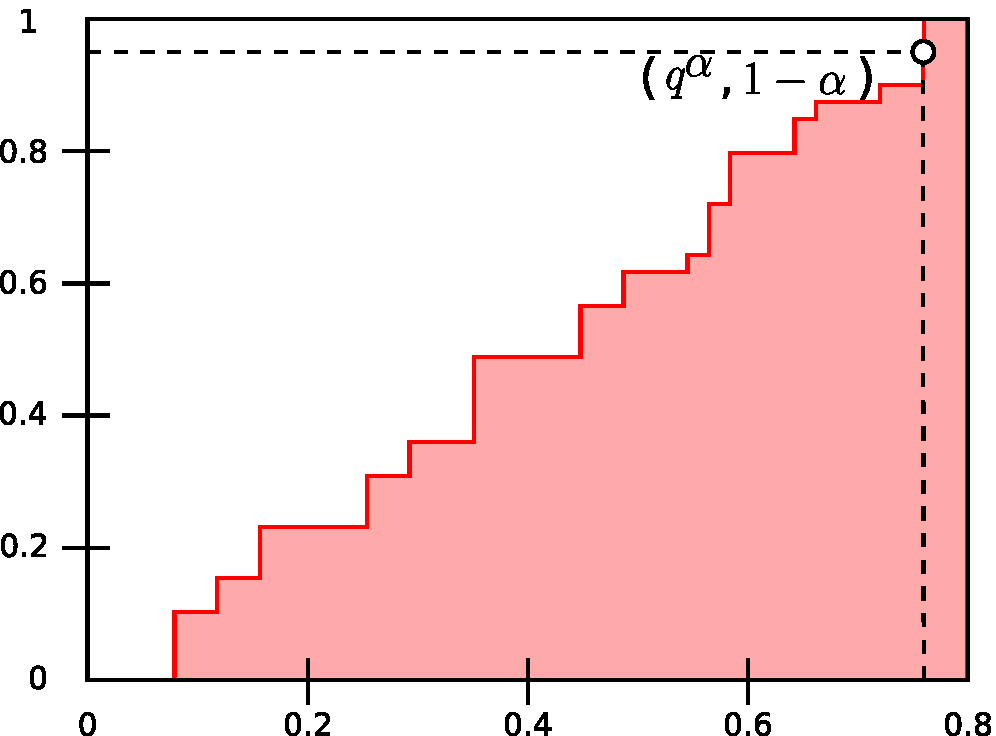
\includegraphics[width=0.75\textwidth]{stat/cdf-discrete}}%
\end{columns}
}

\frame{
\frametitle{Confidence Bands for Landscapes}
\framesubtitle{The Uniform Band}
\begin{columns}
\column{.45\textwidth}
\begin{block}{}
 $$ \ell_n = \bar{\lambda}_n(t) - \frac{\tilde{Z}(\alpha)}{\sqrt{n}}$$
 $$   u_n = \bar{\lambda}_n(t) + \frac{\tilde{Z}(\alpha)}{\sqrt{n}}$$
\end{block}

\column{.45\textwidth}
  \only<1->{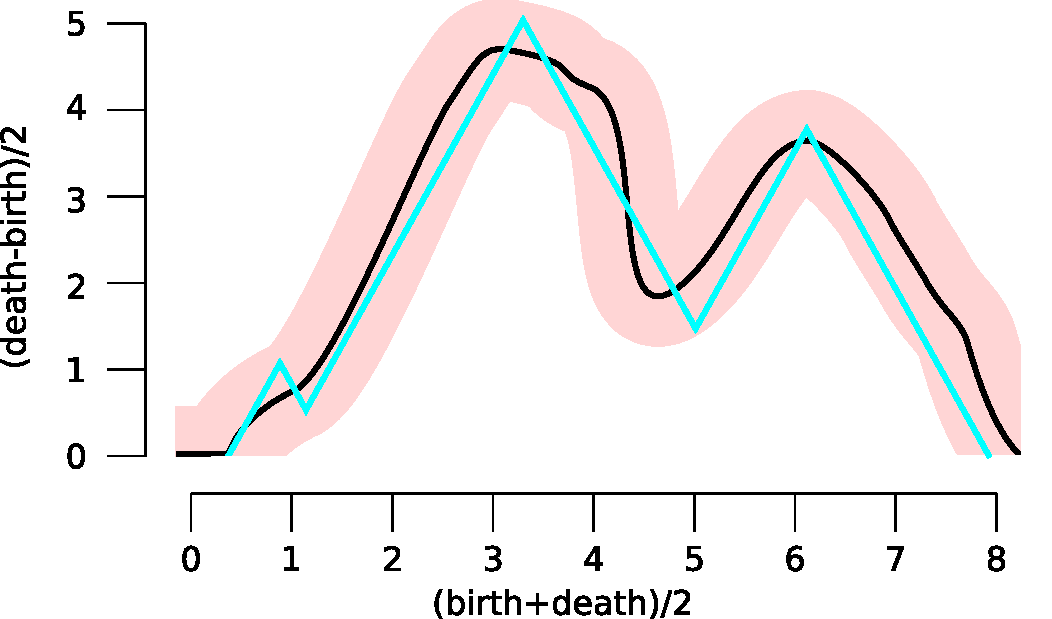
\includegraphics[width=0.75\textwidth]{stat/triangles-CI}}%
\end{columns}

\begin{block}{Uniform Band}
 $$
    \mathbb{P} \left( \ell_n(t) \leq \mu(t) \leq u_n(t)
    \text{ for all } t \right)
    \geq 1 - \alpha
    - \Big( \frac{(\log n)^{\frac{7}{8}} }{n^{\frac{1}{8}}}\Big).
 $$
\end{block}
}

\section{Functional Summaries}
\frame{
\frametitle{Functional Summaries}
\framesubtitle{~}

\begin{block}{}
Here is where I would normally list a bunch of functional summaries, but ...
\end{block}


---------------------------------\\
{Berry, Chen, Cisewski, and Fasy.  One dimensional topological
    descriptors. Preprint available at arXiv:1804.01618.}

}
